\documentclass[twoside]{article}
\setlength{\oddsidemargin}{0 in}
\setlength{\evensidemargin}{0 in}
\setlength{\topmargin}{-0.6 in}
\setlength{\textwidth}{6.5 in}
\setlength{\textheight}{8.5 in}
\setlength{\headsep}{0.75 in}
\setlength{\parindent}{0 in}
\setlength{\parskip}{0.1 in}

\usepackage{url}
\usepackage{titlesec}
\setcounter{secnumdepth}{3}
\usepackage{palatino}
\usepackage{marginnote}
\usepackage{multirow}
\usepackage{easybmat,bigdelim,arydshln}
\usepackage[authoryear,round]{natbib}
\usepackage{amssymb,amsmath,amsthm,amsfonts}
\usepackage{mathtools}
\usepackage{caption}
\usepackage{hyperref}
\usepackage{tcolorbox}
\tcbuselibrary{skins, breakable, theorems}
\usepackage{newpxtext,newpxmath}
\usepackage{longtable}
\usepackage{enumitem}
\makeatletter

\let\bar\overline

\setlist[itemize]{topsep=0pt,leftmargin=10pt,itemsep=-0.2em}
\usepackage{xcolor}
\usepackage{tikz}
\usepackage{pgfplots}
\pgfplotsset{compat = newest}
\usetikzlibrary{patterns,decorations.pathreplacing,decorations.markings}
\usepgfplotslibrary{fillbetween}

\hypersetup{
    colorlinks,
    citecolor=red,
    filecolor=black,
    linkcolor=violet,
    urlcolor=blue
}

\pgfdeclarelayer{ft}
\pgfdeclarelayer{bg}
\pgfsetlayers{bg,main,ft}

\definecolor{myblue}{cmyk}{1,.72,0,.38}
\definecolor{mypurple}{cmyk}{.57,1,0,.58}
\definecolor{myred}{cmyk}{0,.88,.88,.58}
\definecolor{mygreen}{cmyk}{1,0,.69,.66}
\definecolor{myorange}{cmyk}{0,.58,100,.20}

\makeatletter
\renewcommand{\thefigure}{\thesection.\arabic{figure}}
\newtheoremstyle{indented}
  {3pt}% space before
  {3pt}% space after
  {\addtolength{\@totalleftmargin}{3.5em}
   \addtolength{\linewidth}{-3.5em}
   \parshape 1 3.5em \linewidth}% body font
  {}% indent
  {\bfseries}% header font
  {.}% punctuation
  {.5em}% after theorem header
  {}% header specification (empty for default)
\makeatother

\theoremstyle{definition}
\newtheorem{defin}{Definition}[section] % Creates a new counter, number within section
\newtheorem{prt}[defin]{Remark} 
\newtheorem{prts}[defin]{Remarks} % Again share defin's counter
\newtheorem{exmp}[defin]{Example} % etc.
\newtheorem{exmps}[defin]{Examples}
\newtheorem*{note}{Note}
\tcbuselibrary{theorems}

% use counter*=defin to make each tcbtheorem share defin's counter

\newtcbtheorem[use counter*=defin, number within=section]{definition}{Key takeaways}{enhanced, breakable,
    colback = white, colframe = myred, colbacktitle = red!55!black, attach boxed title to top left = {yshift = -2.5mm, xshift = 3mm}, boxed title style = {sharp corners},fonttitle=\bfseries}{takeaway}

\newtcbtheorem[use counter*=defin, number within=section]{theorem}{Theorem}{enhanced, breakable,
    colback = white, colframe = myblue, colbacktitle = blue!45!black, attach boxed title to top left = {yshift = -2.5mm, xshift = 3mm}, boxed title style = {sharp corners},fonttitle=\bfseries}{thm}
    
\newtcbtheorem[use counter*=defin, number within=section]{proposition}{Proposition}{enhanced, breakable,
    colback = white, colframe = teal, colbacktitle = teal, attach boxed title to top left = {yshift = -2.5mm, xshift = 3mm}, boxed title style = {sharp corners},fonttitle=\bfseries}{prop}

\newtcolorbox{example}[1]{enhanced, breakable, colback = white, colframe = orange!85!black, colbacktitle = orange!85!black, attach boxed title to top left = {yshift = -2.5mm, xshift = 3mm}, boxed title style = {sharp corners},fonttitle=\bfseries, title={Example: #1}}

\newtcbox{\myhl}[1][white]
  {on line, arc = 0pt, outer arc = 0pt,
    colback = #1!20!white, colframe = #1!50!black,
    boxsep = 0pt, left = 1pt, right = 1pt, top = 1pt, bottom = 1pt, boxrule = 0pt, bottomrule =0pt, toprule =0pt}
    
\newtcbox{\myhlrule}[1][white]
  {on line, arc = 0pt, outer arc = 0pt,
    colback = #1!20!white, colframe = #1!50!black,
    boxsep = 0pt, left = 1pt, right = 1pt, top = 1pt, bottom = 1pt, boxrule = 0pt, bottomrule =0.5pt, toprule =0.5pt}
%
% The following commands set up the lecnum (lecture number)
% counter and make various numbering schemes work relative
% to the lecture number.
%
\newcounter{lecnum}
\renewcommand{\thepage}{\thelecnum-\arabic{page}}
\renewcommand{\thesection}{\thelecnum.\arabic{section}}
\renewcommand{\theequation}{\thelecnum.\arabic{equation}}
\renewcommand{\thefigure}{\thelecnum.\arabic{figure}}
\renewcommand{\thetable}{\thelecnum.\arabic{table}}

\newcommand{\sidenotes}[1]{\marginnote{\raggedright\scriptsize#1}}
%
% The following macro is used to generate the header.
%
\newcommand{\lecture}[4]{
   \pagestyle{myheadings}
   \thispagestyle{plain}
   \newpage
   \setcounter{lecnum}{#1}
   \setcounter{page}{1}
   \noindent
   \begin{center}
   \framebox{
      \vbox{\vspace{2mm}
    \hbox to 6.28in { {\bf ECON203: Principles of Microeconomics
	\hfill Fall 2022} }
       \vspace{4mm}
       \hbox to 6.28in { {\Large \hfill Note #1: #2  \hfill} }
       \vspace{2mm}
       \hbox to 6.28in { {\it Lecturer: #3 \hfill TA: #4} }
      \vspace{2mm}}
   }
   \end{center}
   \markboth{Week #1: #2}{Week #1: #2}

   {\bf Key points}: {\begin{itemize}
       \item Only the core equations need to be remembered, but don't forget to make sure you understand them first.
       \item You can always try to draw graphs to help you think through the questions, they are our best friend.
   \end{itemize}}

   {\bf Disclaimer}: {\it These notes are written by Sai Zhang for ECON203, based on the problem sets and handouts written by Prof. Brijesh Pinto, the instructor of the course. Please do \textbf{NOT} distribute them online without permission.}
   \vspace*{4mm}
}
%

\tikzset{-stealth-/.style={decoration={
  markings,
  mark=at position #1 with {\arrow{stealth}}},postaction={decorate}}}

  \tikzset{tangent/.style={
    decoration={
        markings,% switch on markings
        mark=
            at position #1
            with
            {
                \coordinate (tangent point-\pgfkeysvalueof{/pgf/decoration/mark info/sequence number}) at (0pt,0pt);
                \coordinate (tangent unit vector-\pgfkeysvalueof{/pgf/decoration/mark info/sequence number}) at (1,0pt);
                \coordinate (tangent orthogonal unit vector-\pgfkeysvalueof{/pgf/decoration/mark info/sequence number}) at (0pt,1);
            }
    },
    postaction=decorate
},
use tangent/.style={
    shift=(tangent point-#1),
    x=(tangent unit vector-#1),
    y=(tangent orthogonal unit vector-#1)
},
use tangent/.default=1}

\begin{document}
\lecture{3}{Questions in PS5-7}{Brijesh Pinto}{Sai Zhang}

\section{Derive and decompose cost}

The section discusses questions in Problem Set 5.

\subsection{Drive cost functions from production functions}

To derive the cost function from a \myhl[blue!45!black]{\textbf{short-run} production function} $F(K,L)$, you can follow the steps below:

\begin{itemize}
    \item \textbf{\underline{Step 1}}: Decide which input is fixed (normally it will be capital $K$), and at which amount
    \item \textbf{\underline{Step 2}}: Given a fixed capital, plug this fixed number into the production function, to get a function of $L$: $F(L)$
    \item \textbf{\underline{Step 3}}: Let this function of $L$ equal to $Q$, and write this function inversely into $L=G(Q)$, that is write labor input $L$ as a function of production $Q$
\end{itemize}

Here are some examples (from Problem Set 5):

\begin{table}[ht]
\centering
    \begin{tabular}{l|ccc}
         production function $F(K,L)$ & $F(K,L)=\sqrt{16+KL}$ & $F(K,L)=\sqrt{KL}$ & $F(K,L)=\frac{L}{5}+\sqrt{KL}$ \\
        \hline
        Step 1: find the fixed input & $K=9$ & $K=2$ & $K=9$ \\
        Step 2: re-write $F(K,L)$ into $F(L)$ & $F(L)=\sqrt{16+9L}$ & $F(L)=\sqrt{9L}=3\sqrt{L}$ & $F(L)=
        \frac{5}{L}+3\sqrt{L}$\\
        Step 3: derive $L=G(Q)$ from $Q=F(L)$ & $L=\frac{Q^2-16}{9}$ & $L=\frac{Q^2}{9}$ & \myhl[red!55!black]{$Q=\frac{5}{L}+3\sqrt{L}$}
    \end{tabular}
\end{table}

several things to keep in mind:
\begin{itemize}
    \item for functions like $F(K,L)=\frac{L}{5}+\sqrt{KL}$, it wouldn't be very easy to do the transformation listed above, don't panic, such questions usually give you a number for $Q$.
    \item Normally, $Q=F(L)$ is an increasing function, that is, more $L$ leads to more $Q$, which means that you can determine
    \begin{itemize}
        \item the minimum quantity $Q_{\min}$ by plug in the minimum value of $L$
        \item the maximum quantity $Q_{\max}$ by plug in the maximum value of $L$
    \end{itemize}
\end{itemize}

\subsection{Decomposition of costs}

First, let's start from the production function $Q=F(K,L)$, still assuming it's a short-term function ($K$ is \textbf{fixed}), and
\begin{itemize}
    \item the price for $K$ (capital rental rate) is $r$
    \item the price for $L$ (wage) is $w$
\end{itemize}

then we have:
$$
\text{Total Cost} = \underbrace{K\cdot r}_{\text{\textbf{Fixed} Cost}} + \underbrace{L\cdot w}_{\text{\textbf{Variable} Cost}}
$$

again, for the examples (let rental rate of capital $r=2$ and wage $w=3$):
\begin{table}[ht]
\centering
    \begin{tabular}{l|cc}
         production function $F(K,L)$ & $F(K,L)=\sqrt{16+KL}$ & $F(K,L)=\sqrt{KL}$ \\
        \hline
        Step 1: find the fixed input & $K=9$ & $K=2$  \\
        Step 2: re-write $F(K,L)$ into $F(L)$ & $F(L)=\sqrt{16+9L}$ & $F(L)=\sqrt{9L}=3\sqrt{L}$ \\
        Step 3: derive $L=G(Q)$ from $Q=F(L)$ & $L=\frac{Q^2-16}{9}$ & $L=\frac{Q^2}{9}$\\
        \hline
        Fixed cost $=K\cdot r$ & $9\times 2=18$ & $2\times 2 =4$\\
        Variable cost $=L\cdot w$ & $L\times 3 = \frac{Q^2-16}{3}$& $L\times 3 = \frac{Q^2}{3}$
    \end{tabular}
\end{table}

In general, the one equation you really need to remember is
\begin{equation}\label{eq:cost_decomp}
    \underbrace{TC}_{\text{total cost}} = \underbrace{FC}_{\text{fixed cost}} + \underbrace{VC}_{\text{variable cost}}
\end{equation}
and if you divide both sides of this equation by $Q$, the quantity of production, you will have
$$
\underbrace{ATC}_{=\frac{TC}{Q},\text{\textbf{average} total cost}} = \underbrace{AFC}_{=\frac{FC}{Q},\text{\textbf{average} fixed cost}} + \underbrace{AVC}_{=\frac{VC}{Q},\text{\textbf{average} variable cost}}
$$
this is the decomposition, remember Equation \ref{eq:cost_decomp}, it's the core equation of this part.

\section{Perfectly Competitive Equilibrium}

Next, we talk about perfectly competitive equilibrium and related problems.

\subsection{Break-even point and shut-down point}

For this type of questions, two things need to be kept in mind:
\begin{itemize}
    \item \textbf{Marginal cost (MC)} line intersect 
    \begin{itemize}
        \item[-] with \textbf{\color{red!55!black}average total cost (ATC)} at ATC line's lowest point
        \item[-] with \textbf{\color{blue!45!black}average variable cost (AVC)} at AVC line's lowest point
    \end{itemize}
    \item[-] In \textbf{perfectly competitive market}, we have 
    $$
    P = MC(Q^*)
    $$
    that is, the marginal cost equals the price in the market at the \textbf{profit-maximizing} quantity $Q^*$.
\end{itemize}

These 2 points give us the graph:

\begin{center}
    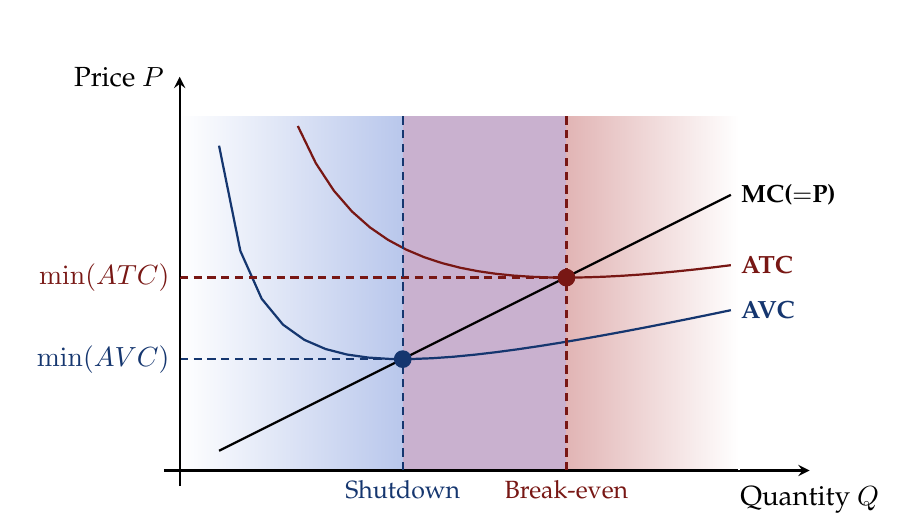
\begin{tikzpicture}[scale=1]
    % basics
    \draw [-stealth,color=black,thick] (-0.2,0) -- (8,0) node[below=2pt] {Quantity $Q$};
    \draw [-stealth,color=black,thick] (0,-0.2) -- (0,5) node[left=2pt] {Price $P$};
    
    \draw[domain=1.5:7, myred, thick, variable=\x] plot ({\x}, {6/\x+\x/4}) node[right] {\small \textbf{ATC}};
    \draw[domain=0.5:7, myblue, thick, variable=\x] plot ({\x}, {2/\x+\x/4}) node[right] {\small \textbf{AVC}};
    \draw[domain=0.5:7, black, thick, variable=\x] plot ({\x}, {\x/2}) node[right] {\small \textbf{MC($=$P)}};
    
    \filldraw[myred] (4.9117,2.4495) circle (3pt); 
    \filldraw[myblue] (2.8329,1.4142) circle (3pt); 
    
    \draw[myred, thick, densely dashed] (0,2.4495) node[left] {$\min(ATC)$}--(4.9117,2.4495);
    \draw[myblue, thick, densely dashed] (0,1.4142) node[left] {$\min(AVC)$}--(2.8329,1.4142);
   
    \draw[name path=BE, myred, thick, densely dashed] (4.9117,0) node[below] {\small Break-even} --(4.9117,4.5);
    \draw[name path=SD, myblue, thick, densely dashed] (2.8329,0) node[below] {\small Shutdown}--(2.8329,4.5);
    \draw[name path=left, black, thick, densely dashed] (0,0)--(0,4.5);
    \draw[name path=right, white!1, thick, densely dashed] (7.1,0)--(7.1,4.5);
    
    \tikzfillbetween[of=SD and left, on layer=bg]{shade, bottom color=myblue!20,top color=white, shading angle =90};
    \tikzfillbetween[of=BE and right, on layer=bg]{shade, bottom color=myred!20,top color=white, shading angle =-90};
    \tikzfillbetween[of=BE and SD, on layer=bg]{color=mypurple!20};
    
\end{tikzpicture}
\end{center}

\begin{itemize}
    \item \textcolor{myblue}{\textbf{\underline{Shutdown}}}: if the price $P$ is \textbf{lower} than the minimal \textcolor{myblue}{\textbf{AVC}} (\myhl[myblue]{$P<\min(AVC)$}, blue-shaded area), the producer loses money for each unit she produces, so she will shut down
    \item \textcolor{myred}{\textbf{\underline{Break-even}}}: if the price $P$ is \textbf{higher} than the minimal \textcolor{myred}{\textbf{ATC}} (\myhl[myred]{$P>\min(ATC)$}, red-shaded area), the produce earns a positive profit, with both fixed cost and variable cost taken into consideration
    \item \textcolor{mypurple}{\textbf{\underline{In-between}}}: if the price $P$ is in-between the two points (\myhl[mypurple]{$\min(AVC)<P<\min(ATC)$}, purple-shaded area), for each unit produced, the producer earn some money, so she will \textbf{continue}; but still not covering the fixed cost, hence earns a \textbf{negative profit}
\end{itemize}

\subsection{Competitive equilibrium and welfare}
The most important thing to do to solve questions similar to those in PS6 is to draw the graph, and transform the question into a geometric problem. Let's break down the steps:

\begin{itemize}
    \item \textbf{\underline{Step 1}}: determine the equilibrium price, i.e., solve the system of equations of demand and supply.
\end{itemize}

\begin{center}
    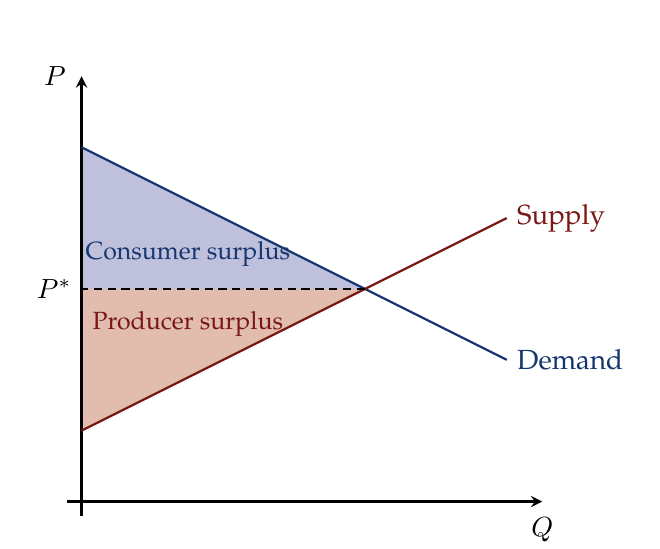
\begin{tikzpicture}[scale=0.9]
        % basics
        \draw [-stealth,color=black,thick] (-0.2,0) -- (6.5,0) node[below=2pt] {$Q$};
        \draw [-stealth,color=black,thick] (0,-0.2) -- (0,6) node[left=2pt] {$P$};
        
        \draw[name path=D, domain=0:6, myblue, thick, variable=\x] plot ({\x}, {5-\x/2}) node[right] {Demand};
        \draw[name path=S, domain=0:6, myred, thick, variable=\x] plot ({\x}, {1+\x/2}) node[right] {Supply};
        
        \draw[name path=eqbm, densely dashed, black, thick] plot (4,3)--(0,3) node[left] {$P^*$};
        
        \tikzfillbetween[of=D and eqbm, on layer=bg]{myblue!20};
        \tikzfillbetween[of=S and eqbm, on layer=bg]{myred!20};
        
        \node[align=left, myblue] at (1.5,3.5) {\small Consumer surplus};
        \node[align=left, myred] at (1.5,2.5) {\small Producer surplus};
        
    \end{tikzpicture}
\end{center}

\begin{itemize}
    \item \textbf{\underline{Step 2}}: Examine how a policy bounds the market away from the equilibrium point.
\end{itemize} 

\subsubsection*{Price control policies}
For price control policies, follow these steps
\begin{center}
\begin{minipage}[b]{0.45\textwidth}
    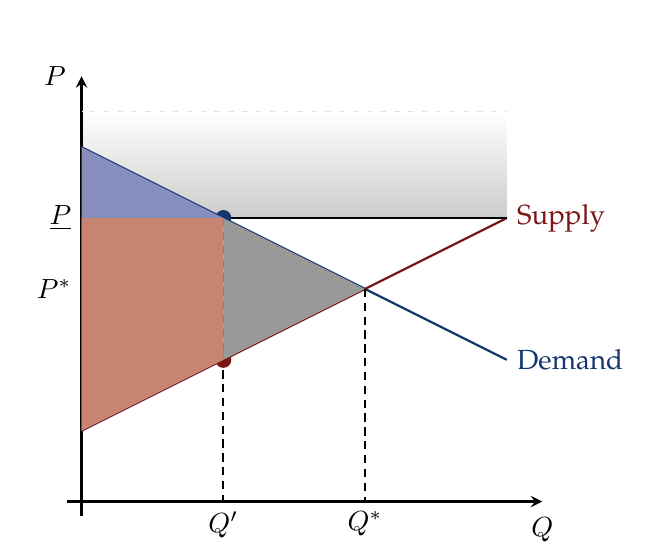
\begin{tikzpicture}[scale=0.9]
        % basics
        \draw [-stealth,color=black,thick] (-0.2,0) -- (6.5,0) node[below=2pt] {$Q$};
        \draw [-stealth,color=black,thick] (0,-0.2) -- (0,6) node[left=2pt] {$P$};
        
        \draw[name path=D1_1, myblue, thick] (0,5)--(2,4);
        \draw[name path=D1_2, domain=2:4, myblue, thick, variable=\x] plot ({\x}, {5-\x/2});
        \draw[name path=D1_3, domain=4:6, myblue, thick, variable=\x] plot ({\x}, {5-\x/2}) node[right] {Demand};
        \draw[name path=S1_1, domain=0:2, myred, thick, variable=\x] plot ({\x}, {1+\x/2});
        \draw[name path=S1_2, domain=2:4, myred, thick, variable=\x] plot ({\x}, {1+\x/2});
        \draw[name path=S1_3, domain=4:6, myred, thick, variable=\x] plot ({\x}, {1+\x/2}) node[right] {Supply};
        \draw[name path=down, densely dashed, black, thin] plot (0,0)--(6,0);
        
        \draw[name path=eqbm1d, densely dashed, black, thick] plot (2,3)--(0,3) node[left] {$P^*$};
        \draw[name path=eqbm1, densely dashed, black, thick] plot (4,3)--(2,3);
        \draw[name path=eqbm1quant, densely dashed, black, thick] plot (4,3)--(4,0) node[below] {$Q^*$};
        \draw[name path=up, densely dashed, white, thin] plot (0,5.5)--(6,5.5);
        \draw[black, thick, densely dashed] plot (2,4) -- (2,0) node[below] {$Q^{\prime}$};
        
        \draw[name path=pfloor, black, thick] plot (0,4) node[left] {$\underline{P}$}--(6,4);
        \draw[name path=pfloord, black, thick] plot (2,4) --(0,4);
        \filldraw[myblue] (2,4) circle (3pt);
        \filldraw[myred] (2,2) circle (3pt);
        
        \tikzfillbetween[of=S1_1 and D1_1, on layer=ft]{myblue!40};
        \tikzfillbetween[of=pfloord and S1_1, on layer=ft]{myred!40};
        \tikzfillbetween[of=D1_2 and S1_2, on layer=ft]{black!40};
        
        \tikzfillbetween[of=pfloor and up, on layer=bg]{shade, bottom color=black!20,top color=white, shading angle =0};
        
        
        %\tikzfillbetween[of=S and eqbm, on layer=bg]{myred!20};
        
    \end{tikzpicture}
  \end{minipage}
  \hfill
  \begin{minipage}[b]{0.45\textwidth}
    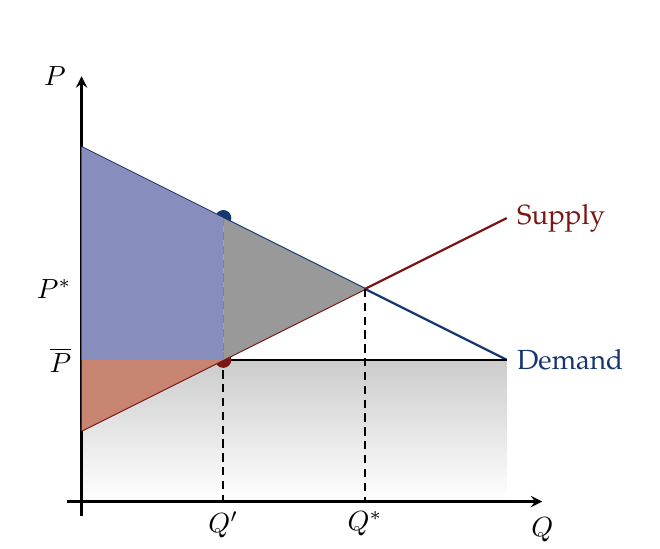
\begin{tikzpicture}[scale=0.9]
        % basics
        \draw [-stealth,color=black,thick] (-0.2,0) -- (6.5,0) node[below=2pt] {$Q$};
        \draw [-stealth,color=black,thick] (0,-0.2) -- (0,6) node[left=2pt] {$P$};
        
        \draw[name path=D2_1, domain=0:2, myblue, thick, variable=\x] plot ({\x}, {5-\x/2});
        \draw[name path=D2_2, domain=2:4, myblue, thick, variable=\x] plot ({\x}, {5-\x/2});
        \draw[name path=D2_3, domain=4:6, myblue, thick, variable=\x] plot ({\x}, {5-\x/2}) node[right] {Demand};
        \draw[name path=S2_1, domain=0:2, myred, thick, variable=\x] plot ({\x}, {1+\x/2});
        \draw[name path=S2_2, domain=2:4, myred, thick, variable=\x] plot ({\x}, {1+\x/2});
        \draw[name path=S2_3, domain=4:6, myred, thick, variable=\x] plot ({\x}, {1+\x/2}) node[right] {Supply};
        \draw[name path=down, densely dashed, black, thin] plot (0,0)--(6,0);
        \draw[black, thick, densely dashed] plot (2,4) -- (2,0) node[below] {$Q^{\prime}$};
        
        \draw[name path=eqbm2d, densely dashed, black, thick] plot (2,3)--(0,3) node[left] {$P^*$};
        \draw[name path=eqbm2, densely dashed, black, thick] plot (4,3)--(2,3);
        \draw[name path=eqbm2quant, densely dashed, black, thick] plot (4,3)--(4,0) node[below] {$Q^*$};
        
        \draw[name path=pceil, black, thick] plot (0,2) node[left] {$\bar{P}$}--(6,2);
        \draw[name path=pceild, black, thick] plot (2,2) --(0,2);
        
        \filldraw[myblue] (2,4) circle (3pt);
        \filldraw[myred] (2,2) circle (3pt);
        
        \tikzfillbetween[of=D2_1 and S2_1, on layer=ft]{myred!40};
        \tikzfillbetween[of=D2_1 and pceild, on layer=ft]{myblue!40};
        \tikzfillbetween[of=D2_2 and S2_2, on layer=ft]{black!40};
        
        \tikzfillbetween[of=pceil and down, on layer=bg]{shade, bottom color=white,top color=black!20, shading angle =0};
        
    \end{tikzpicture}
  \end{minipage}
\end{center}

First, for price control policies:
\begin{itemize}
    \item[\textbf{S1}] determine whether the policy actually makes a difference:
    \begin{itemize}
        \item[-] for a \textbf{price floor} $\underline{P}$ to have an impact: $\underline{P}>P^*$, that is, price floor is higher than the equilibrium price.
        \item[-] for a \textbf{price ceiling} $\bar{P}$ to have an impact: $\bar{P}<P^*$, that is, price floor is lower than the equilibrium price.
    \end{itemize}
    The impact for both is \textbf{reducing the quantity} traded in the market, from $Q^*$ to $Q^{\prime}$
    \item[\textbf{S2}] Next, use either $\underline{P}$ or $\bar{P}$ to calculate the post-policy trading quantity $Q'$
    \item[\textbf{S3}] Then, recalculate the surplus:
    \begin{itemize}
        \item[-] \textbf{\color{myblue}Consumer Surplus \textit{(in blue)}}: Consumer surplus is the area determined by \myhl[myblue]{$Q=0$}, post-price-policy Q (\myhl[myblue]{$Q^{\prime}$}), the restricted price (either \myhl[myblue]{$\underline{P}$ or $\bar{P}$}) and the \myhl[myblue]{demand curve}. 
        \item[-] \textbf{\color{myred}Producer Surplus \textit{(in red)}}: Producer surplus is the area determined by \myhl[myred]{$Q=0$}, post-price-policy Q (\myhl[myred]{$Q^{\prime}$}), the restricted price (either \myhl[myred]{$\underline{P}$ or $\bar{P}$}) and the \myhl[myred]{supply curve}. 
        \item[-] \textbf{Deadweight Lost \textit{(in grey)}}: Because the quantity traded is now $Q'$, smaller than the equilibrium quantity $Q^*$, there is a deadweight lost\footnote{Understand it this way: the deadweight lost is the wasted potential of the market due to the price control policy.}, which is the triangular area determined by \underline{post-price policy Q($Q'$)}, the \underline{demand curve} and the \underline{supply curve}.
    \end{itemize}
\end{itemize}

Now, the question is transformed into a geometry question, it should be easy and clear to solve :)

\subsubsection*{Unit tax}

Another policy to consider is the unit tax. With this policy, it's better to start numerically:

For a demand curve:
$$
P = a-mQ
$$
and a supply curve:
$$
P = b+nQ
$$
a unit tax of $t$ per unit of quantity:
$$
t
$$
then, use this formula to solve the post tax quantity $Q^{tax}$:
$$
a-mQ - (b+nQ) = t
$$

take Q8 of PS6 as an example: we have
$$\begin{aligned}
    P&= 12-Q & \text{demand}\\
    P&= 2+Q & \text{supply}\\
    t& =4 & \text{unit tax rate}
\end{aligned} \Rightarrow 12-Q-(2+Q)=4\Rightarrow Q^{tax}=3
$$

then you can proceed with this following graph to understand the components of welfare:

\begin{center}
    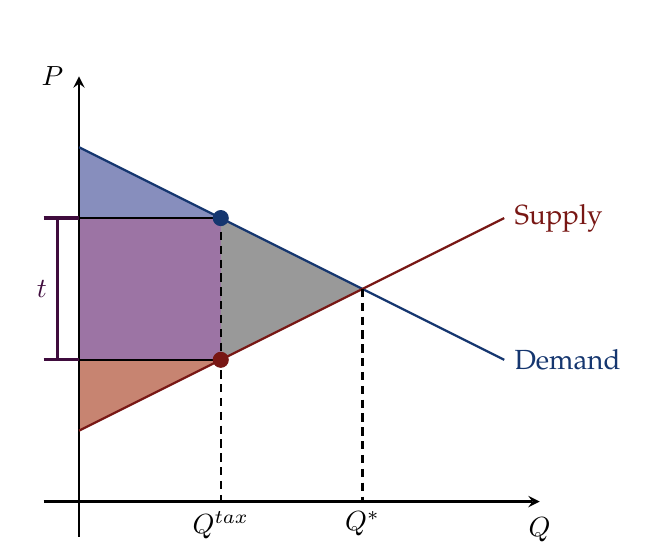
\begin{tikzpicture}[scale=0.9]
        % basics
        \draw [-stealth,color=black,thick] (-0.5,0) -- (6.5,0) node[below=2pt] {$Q$};
        \draw [-stealth,color=black,thick] (0,-0.5) -- (0,6) node[left=2pt] {$P$};
        
        \draw[name path=D3_1, domain=0:2, myblue, thick, variable=\x] plot ({\x}, {5-\x/2});
        \draw[name path=D3_2, domain=2:4, myblue, thick, variable=\x] plot ({\x}, {5-\x/2});
        \draw[name path=D3_3, domain=4:6, myblue, thick, variable=\x] plot ({\x}, {5-\x/2}) node[right] {Demand};
        \draw[name path=S3_1, domain=0:2, myred, thick, variable=\x] plot ({\x}, {1+\x/2});
        \draw[name path=S3_2, domain=2:4, myred, thick, variable=\x] plot ({\x}, {1+\x/2});
        \draw[name path=S3_3, domain=4:6, myred, thick, variable=\x] plot ({\x}, {1+\x/2}) node[right] {Supply};
        \draw[name path=down, densely dashed, black, thin] plot (0,0)--(6,0);
        \draw[black, thick, densely dashed] plot (2,4) -- (2,0) node[below] {$Q^{tax}$};
        
        \draw[name path=eqbm2quant, densely dashed, black, thick] plot (4,3)--(4,0) node[below] {$Q^*$};
        
        \draw[name path=pceil, black, thick] plot (2,2) --(0,2);
        \draw[name path=pfloor, black, thick] plot (2,4) --(0,4);
        
        \draw[mypurple, very thick] plot (-0.3,2) -- node[left] {$t$} (-0.3,4);
        \draw[mypurple, very thick] plot (-0.5,2) -- (0,2);
        \draw[mypurple, very thick] plot (-0.5,4) -- (0,4);
        
        \filldraw[myblue] (2,4) circle (3pt);
        \filldraw[myred] (2,2) circle (3pt);
        
        \tikzfillbetween[of=D3_1 and pfloor, on layer=bg]{myblue!40};
        \tikzfillbetween[of=S3_1 and pceil, on layer=bg]{myred!40};
        \tikzfillbetween[of=pfloor and pceil, on layer=bg]{mypurple!40};
        \tikzfillbetween[of=D3_2 and S3_2, on layer=bg]{black!40};
        
    \end{tikzpicture}
\end{center}

\begin{itemize}
\item[-] \textbf{\color{myblue}Consumer Surplus \textit{(in blue)}} 
\item[-] \textbf{\color{myred}Producer Surplus \textit{(in red)}} 
\item[-] \textbf{Deadweight Lost \textit{(in grey)}}
\item[-] \textbf{\color{mypurple}Tax (\textit(government surplus)}: $T=t\cdot Q^{tax}$
\end{itemize}

Easy!

\section{Monopoly}
In a monopoly setting, you can follow these steps for the questions like the ones in PS7.

\begin{itemize}
    \item \textbf{\underline{Step 1}}: Find out the marginal cost (\myhl[myblue]{\textbf{MC(Q)}}) and marginal revenue (\myhl[myred]{\textbf{MR(Q)}})
    \begin{itemize}
        \item[-] \myhl[myblue]{\textbf{MC(Q)}}: there will be 2 scenarios
        \begin{itemize}
            \item[1.] you are given the formula of $MC(Q)$ (like Q2-6 of PS7): You can just use this formula and proceed.
            \item[2.] you are given the total cost curve $C(Q)$ (like Q7-10 of PS7):  take the \textbf{derivative} of $C(Q)$ with respect to $Q$ to get the marginal cost function.
        \end{itemize}
        \item[-] \myhl[myred]{\textbf{MR(Q)}}: for a demand curve $P=a-mQ$, the marginal revenue is $MR(Q)=a-2mQ$
    \end{itemize}
    \item \textbf{\underline{Step 2}}: Determine of optimal quantity $Q^*$, depending on what the producer tries to maximize: 
    \begin{itemize}
        \item[-] \textbf{\underline{profit}-maximizing}: solve $Q$ from $MC(Q)=MR(Q)$
        \item[-] \textbf{\underline{revenue}-maximizing}: solve $Q$ from $MR(Q)=0$
        \item[-] \textbf{\underline{cost}-minimizing} (rarely seen): solve $Q$ from $MC(Q)=0$
    \end{itemize}
    
    \item \textbf{\underline{Step 3}}: calculate what is required to be calculated, which could be
    \begin{itemize}
        \item[-] \textbf{price}: plug the optimal quantity $Q^*$ back into the \textbf{demand curve} $P^*=a-mQ^*$ 
        \item[-] \textbf{revenue}: price times quantity $R^* = P^*\cdot Q^*$
        \item[-] \textbf{cost}: plug the quantity back into the total cost function $C(Q^*)$
        \item[-] \textbf{profit}: revenue minus cost $R^*-C(Q^*)$
    \end{itemize}
\end{itemize}

See, not that difficult!

\vspace{20pt}
\noindent\rule{\textwidth}{0.4pt}

\textbf{Some examples of derivatives}
\begin{table}[ht]
\centering
    \begin{tabular}{cc}
         Function & Derivative\\
        \hline
        $f(x)=ax$ & $f'(x)=a$\\
        $f(x)= x^b$ & $f'(x)=bx^{b-1}$\\
        $f(x) =e^x$ & $f'(x)=e^x$\\
        $f(x)=\ln(x)$ & $f'(x)=\frac{1}{x}$
    \end{tabular}
\end{table}

these are the examples that we are mostly likely to encounter, and here is a nice \href{https://www.mathsisfun.com/calculus/derivatives-rules.html}{reference}.

%\newpage
%\bibliographystyle{plainnat}
%\bibliography{ref.bib}

\end{document}